\documentclass{beamer}
\usepackage[utf8]{inputenc}

\usetheme{Madrid}
\usecolortheme{default}
\usepackage{amsmath,amssymb,amsfonts,amsthm}
\usepackage{txfonts}
\usepackage{tkz-euclide}
\usepackage{listings}
\usepackage{adjustbox}
\usepackage{array}
\usepackage{tabularx}
\usepackage{gvv}
\usepackage{lmodern}
\usepackage{circuitikz}
\usepackage{tikz}
\usepackage{graphicx}
\usepackage{amsmath}

\setbeamertemplate{page number in head/foot}[totalframenumber]

\usepackage{tcolorbox}
\tcbuselibrary{minted,breakable,xparse,skins}



\definecolor{bg}{gray}{0.95}
\DeclareTCBListing{mintedbox}{O{}m!O{}}{%
  breakable=true,
  listing engine=minted,
  listing only,
  minted language=#2,
  minted style=default,
  minted options={%
    linenos,
    gobble=0,
    breaklines=true,
    breakafter=,,
    fontsize=\small,
    numbersep=8pt,
    #1},
  boxsep=0pt,
  left skip=0pt,
  right skip=0pt,
  left=25pt,
  right=0pt,
  top=3pt,
  bottom=3pt,
  arc=5pt,
  leftrule=0pt,
  rightrule=0pt,
  bottomrule=2pt,
  toprule=2pt,
  colback=bg,
  colframe=orange!70,
  enhanced,
  overlay={%
    \begin{tcbclipinterior}
    \fill[orange!20!white] (frame.south west) rectangle ([xshift=20pt]frame.north west);
    \end{tcbclipinterior}},
  #3,
}
\lstset{
    language=C,
    basicstyle=\ttfamily\small,
    keywordstyle=\color{blue},
    stringstyle=\color{orange},
    commentstyle=\color{green!60!black},
    numbers=left,
    numberstyle=\tiny\color{gray},
    breaklines=true,
    showstringspaces=false,
}


\title 
{5.3.15}
\date{September 27,2025}


\author 
{Abhiram Reddy-AI25BTECH11021}



\begin{document}


\frame{\titlepage}

% Frame: Question
\begin{frame}{Question 5.3.15}
What type of lines will you get by drawing the graph of the pair of equations:
\[
x - 2y + 3 = 0 \quad \text{and} \quad 2x - 4y = 5?
\]
\end{frame}

% Frame: Step 1
\begin{frame}{Step 1: Convert to Standard Form}
Write both equations in the standard form:
\begin{equation}
x - 2y = -3
\label{eq:1}
\end{equation}
\begin{equation}
2x - 4y = 5
\label{eq:2}
\end{equation}
We can represent them in matrix-vector form:
\begin{equation}
\mathbf{A} = \begin{bmatrix} 1 & -2 \\ 2 & -4 \end{bmatrix}, \quad
\mathbf{x} = \begin{bmatrix} x \\ y \end{bmatrix}, \quad
\mathbf{b} = \begin{bmatrix} -3 \\ 5 \end{bmatrix}
\end{equation}
Then the system becomes:
\begin{equation}
\mathbf{A} \mathbf{x} = \mathbf{b}
\end{equation}
\end{frame}

% Frame: Step 2
\begin{frame}{Step 2: Analyze the System}
Observe the coefficient matrix:
\[
\mathbf{A} = \begin{bmatrix} 1 & -2 \\ 2 & -4 \end{bmatrix}
\]
We see:
\begin{equation}
\text{Row}_2 = 2 \times \text{Row}_1
\end{equation}
This implies the equations are **linearly dependent** in coefficients.

Now check the constants:
\begin{equation}
c_2 = 5 \neq 2 \times c_1 = 2 \times (-3) = -6
\end{equation}
So the constants are not in the same ratio as the coefficients.
\end{frame}

% Frame: Step 3
\begin{frame}{Step 3: Matrix Rank and Conclusion}
The augmented matrix is:
\[
\left[
\begin{array}{cc|c}
1 & -2 & -3 \\
2 & -4 & 5
\end{array}
\right]
\]

Then:
\begin{equation}
\text{rank}(\mathbf{A}) = 1, \quad \text{rank}(\mathbf{A}|\mathbf{b}) = 2
\end{equation}

Therefore, the system is:
\[
\boxed{
\text{Inconsistent (no solution)}
}
\]

\[
\Rightarrow \boxed{
\text{Lines are parallel and distinct}
}
\]
\end{frame}

% Frame: C Code
\begin{frame}[fragile]{C Code to Determine Line Relationship}
\begin{lstlisting}[language=C]
#include <stdio.h>
#include <stdbool.h>

bool areEqual(double a, double b, double epsilon) {
    return (a - b < epsilon) && (b - a < epsilon);
}

int main() {
    double a1 = 1, b1 = -2, c1 = -3;
    double a2 = 2, b2 = -4, c2 = 5;

    double ratio_a = a1 / a2;
    double ratio_b = b1 / b2;
    double ratio_c = c1 / c2;

    double epsilon = 1e-6;

    if (areEqual(ratio_a, ratio_b, epsilon) && !areEqual(ratio_b, ratio_c, epsilon)) {
        printf("The lines are parallel and distinct.\n");
    } else if (areEqual(ratio_a, ratio_b, epsilon) && areEqual(ratio_b, ratio_c, epsilon)) {
        printf("The lines are coincident.\n");
    } else {
        printf("The lines intersect (are not parallel).\n");
    }

    return 0;
}
\end{lstlisting}
\end{frame}





\begin{frame}[fragile]{Python Code: Plotting the Graphs}
    \framesubtitle{Visualization of the Locus and an Example Line}
    
    \lstset{style=PythonStyle}
    \begin{lstlisting}[language=Python]
import matplotlib.pyplot as plt
import numpy as np

# 1. Define the range for x
x = np.linspace(-10, 10, 400)

# 2. Define the equations in slope-intercept form (y = mx + b)
# Equation 1: y = (1/2)x + 3/2
y1 = (1/2) * x + 3/2

# Equation 2: y = (1/2)x - 5/4
y2 = (1/2) * x - 5/4

# 3. Create the plot
plt.figure(figsize=(8, 6))

# Plot the lines
plt.plot(x, y1, label='$x - 2y + 3 = 0$ ($y = 0.5x + 1.5$)', color='blue')
plt.plot(x, y2, label='$2x - 4y = 5$ ($y = 0.5x - 1.25$)', color='red', linestyle='--')

# 4. Customize the plot
plt.title('Graph of a Pair of Linear Equations (Parallel Lines)')
plt.xlabel('x-axis')
plt.ylabel('y-axis')
plt.axhline(0, color='black', linewidth=0.5) # x-axis line
plt.axvline(0, color='black', linewidth=0.5) # y-axis line
plt.grid(color='gray', linestyle=':', linewidth=0.5)
plt.legend()
plt.axis('equal') # Ensures that the slopes look correct
plt.show()
plt.savefig('python_plot.png')
    \end{lstlisting}
\end{frame}

\begin{frame}{Plot}
    \centering
    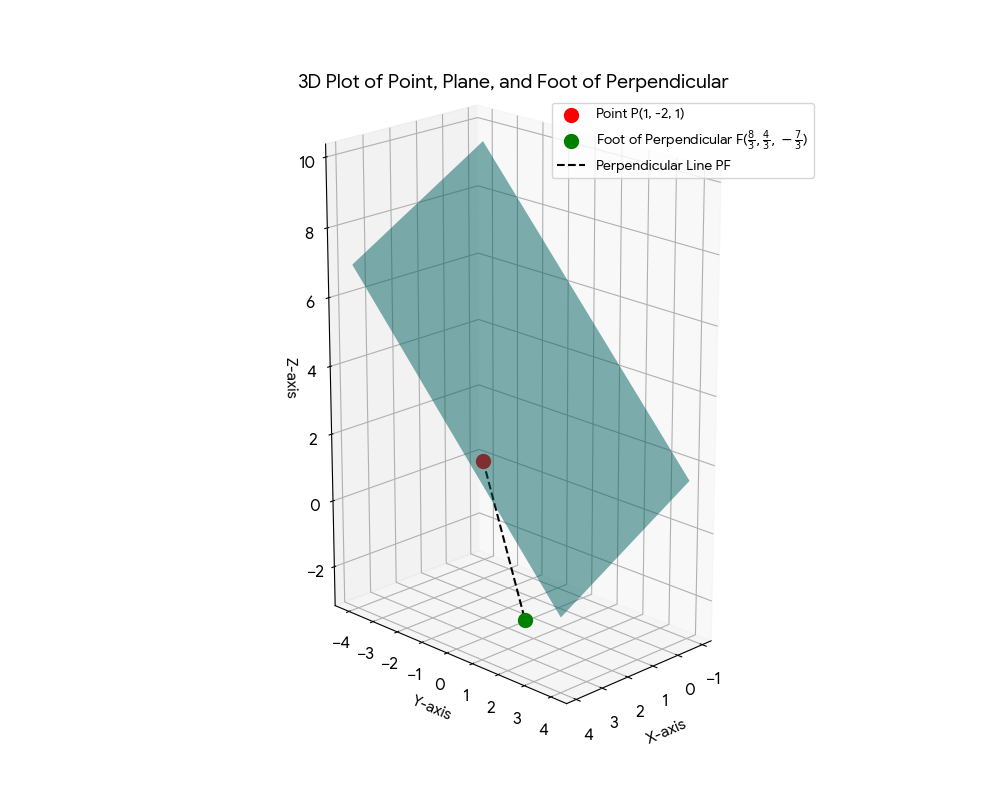
\includegraphics[width=\columnwidth, height=0.8\textheight, keepaspectratio]{figs/python_plot.png}     
\end{frame}


\end{document}